\documentclass{article}
\usepackage[utf8]{inputenc}
\usepackage{graphicx}
\usepackage{hyperref}
\usepackage{amsmath}
\graphicspath{{images/}}
\title{EVM Model(COP290-Design Practices)}
\author{Shreshth Tuli$^{1}$}
\date{April 2018}

\begin{document}

\maketitle
\footnotetext[1]{This document and model have been developed after collective discussion and sharing ideas with Sankalan Pal Chowdhury}
\section{Motivation}
Elections are the backbone of any representative democracy. Elections have been existent since the Roman times, and have seen many changes over the centuries. In the most recent form, most of the process has been digitized with the use of Electronic Voting Machines(EVMs). For the Indian General Elections, these are currently designed by Bharat Electronics and Electronics Corporation of India.

Elections can broadly be categorized into open ballot and secret ballot. while open ballot elections are rarely an issue, secret ballot elections are much more complicated since there is a question of secrecy involved. Even in the digital era, a provably free and fair election has not become a possibility. In this article we look at some properties that an ideal EVM should have. We then propose our own model of a design of an EVM which tries to satisfy these properties.
\section{Model Requirements}
The ideal model for a vote collection and counting software must include at least the following properties:
\subsection{Coercion Freedom}
The purpose of conducting a vote in any democracy is to ensure that the people in power are the people who the population wants to be in power. An inherent assumption in this process is that each persons vote reflects their independent personal choice, and not a reflection of some threat or external influence. While physical coercion is something that other democratic institutions must prevent, we must make sure that there are no loopholes in our design that breaks down this condition
\subsection{Secrecy}
The Constitution of India, and most other representative democracies specify that elections are supposed to be secret ballots. Maintaining the secrecy of who  a certain voter votes for is also important for maintaining the coercion freedom since anyone attempting to coerce a voter would like to figure out if it worked.\newline

Secrecy therefore becomes an utmost requirement for any vote collecting model. The problem is not at all trivial, since, on one hand, individual votes need to be kept secret, but on the other hand, aggregate measures need to be reveled for the purpose of declaring results. This gives rise to a very important question:\textit{What is the minimum number of voters for whom the aggregate counts can be revealed?} 
\subsection{Non-Repudiation}
Keeping a vote secret however should not imply opacity of the process. If a vote once caste is lost into the world of cryptography, then it is likely that the losing candidates will cry foul. Therefore it is important that once a voter castes a vote in someones favor, it is binding upon them. Should they claim to have voted differently than what the result implies, there should be a mechanism to prove their claims false. This is Non-Repudiation.\newline

At this point it is important to note that Non-Repudiation and Secrecy already seem to contradict each other. The logical way to deal with this is to reveal some limited information about the vote caste by a voter that proves that his vote was counted, but does not reveal who he voted for. 
\subsection{Audit ability}
While Non-Repudiation makes sure that a significant number of voters cannot cry foul, one also needs to have a mechanism to convince the candidates that the result outputted by the system is really what the voters wanted it to be. Therefore, there needs to be a mechanism to audit the entire process of voting, while not revealing any information about individual votes(This is different from the Non-Repudiation case where the voters agree to their votes being revealed). Further, if there is any probabilistic component in the design(Which is rather common in Cryptography systems), there needs to be a way to show that it does not introduce any bias towards one party.
\subsection{Anonymity}
Anonymity is somewhat related to Secrecy, and would generally not require additional constructs, but it is still important to understand the difference: Secrecy implies that \textit{given a set of voters smaller than a prescribed limit, no one should be able to say with certainty how many of them voted for which candidate.} Anonymity, on the other hand is the requirement that \textit{given a certain candidate, one should not be able to identify the set of voters who voted for them.}  
\subsection{Verifiable}
While a system may claim to have several desirable properties, it does not have any worth unless there is a mathematically rigorous model that can prove all these claims. Therefore any system that we propose must be backed by a mathematical model which is both concrete and accessible to anyone who wishes to see it.
\subsection{Self-Certifiable}
Once the system has been deemed to be satisfactory, and verified mathematically, it needs to be deployed. This final step however can lead to doubts on whether the deployed version is same as the proposed version. Should that be the case, all the previous steps become useless. Therefore, there needs to be a way to test the integrity of the hardware, software and firmware at every stage of deployment.

\section{Assumptions Made}
In our model, we make the following Assumptions:
\begin{itemize}
    \item \textbf{Literacy: }While India is definitely quite far from universal literacy, it is definitely making progress towards it. In our present model, we need the user to be literate in order to verify their vote. Note that this is not a requirement in order to caste their vote.
    \item \textbf{Biometric Data: }The Unique Identification Project in India aims to create a database of biometric data for all the residents of India. Also, the process of linking Voter ID cards to the UID card has already started. While there are considerable issues with this project as of now, we assume that a linked universal biometric database will be achieved and be made available for the purpose of elections.
    \item \textbf{Physical Security: }Any technological model must rely on the fact that it will be free of physical attacks on itself as well as its users, eg. if an adversary is able to place an observer in the polling booth, then no technology can provide secrecy.Same is the case for cracking n the devices to some extent. We assume that the law enforcement agencies will be able to handle such problems.
    
\end{itemize}

\section{Relevant Concepts}
\subsection{One Time Pad}
In cryptography, the one-time pad (OTP) is an encryption technique that cannot be cracked, but requires the use of a one-time pre-shared key the same size as, or longer than, the message being sent. In this technique, a plaintext is paired with a random secret key. Then, each bit or character of the plain text is encrypted by combining it with the corresponding bit or character from the pad using modular addition. For binary case, this is simply the XOR of the two texts.

The idea of OTP can easily be extended to any base. We seek to make use of it to provide for non-repudiation. Suppose there are n candidates contesting for a given seat. These candidates are indexed [0,...,n-1]. Now suppose two votes are recorded, one of these being the actual vote($k_{v1}$), and the other being the key to encrypt it with($k_{v2}$). We calculate the \textbf{vote sum($k_{vs}$)} of these using $$k_{vs}=k_{v1}+k_{v2} \mod n$$

It is easy to prove that while knowing both quantities on the LHS lets us determine the RHS uniquely, the RHS gives no clue about the individual quantities on the LHS. This is true because for any $k_{v1}=p$ and $k_{vs}=q$, we can choose $k_{v2}=q-p \mod{n}$. So, if the test vote is used as a key, then it is always okay to display the vote sum to the public for the purpose of non-repudiability.

\subsection{Dynamic RAM}
Dynamic RAMS are semiconductor chips in which each bit of memory data is stored as the presence or absence of an electric charge on a small capacitor on the chip. As time passes, the charges in the memory cells leak away, so without being refreshed the stored data would eventually be lost. To prevent this, external circuitry periodically reads each cell and rewrites it, restoring the charge on the capacitor to its original level.

An important property of these DRAMS is that in order to read the value stored in a cell, one must drain the capacitor which holds it, in effect wiping off the data. This is known as destructive read. In a general purpose RAM, there would be additional circuitry to restore the data that has been read, but we wish to use this destructive read property to our benefit in our proposed design.
\subsection{Fingerprint Science}
A fingerprint in its narrow sense is an impression left by the friction ridges of a human finger. Human fingerprints are detailed, nearly unique, difficult to alter, and durable over the life of an individual, making them suitable as long-term markers of human identity.

(British) India was one of the first countries to begin the use of fingerprints as Identification by sir William Hershell in 1877. Even 150 years later, India continues to be in the forefront for using biometrics to identify people(Similar initiatives exist in only 4 other countries). In our proposed solution, we wish to use Fingerprints as a way of authenticating voters. 
\section{Proposed Model}
An overview of our design of EVM is given in the block diagram below. Descriptions of each of the four units is given after that.  \newline
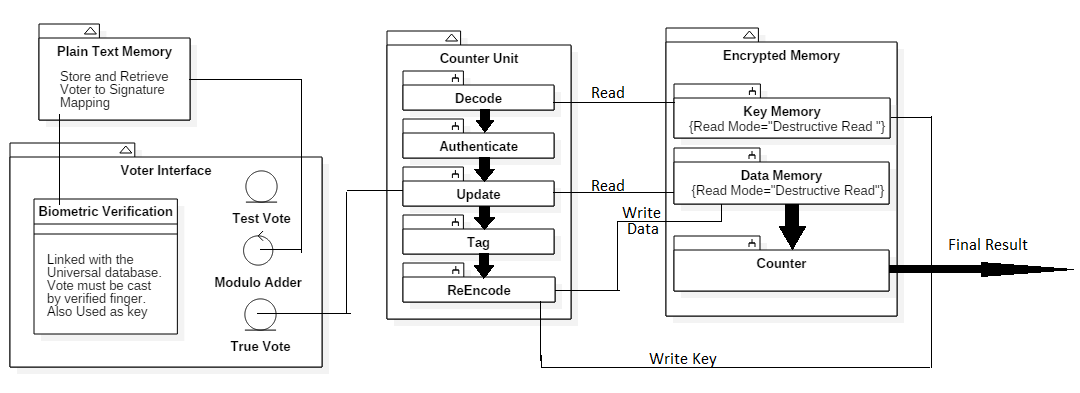
\includegraphics[width=\textwidth]{EVM_Model}

\subsection{Voter Interface}
This is the user interface of the EVM, which we plan to keep more or less similar to the present design, with the exception that each button needs to be fit with a fingerprint scanner. This is a cross verification step that would augment the existing verification, so a reasonable false positive rate can be accepted, but we need to completely avoid false negatives. 

The voter needs to first press a button, in order to verify that the machine is working correctly(ie if the corresponding LED is lighting up). This button press has no effect on the actual voting procedure. Once the voter has verified, they need to cast their real vote. The value of the real vote is sent over to the Counter Unit. On The Plain Text memory is sent the key obtained from the fingerprint(this can be done in multiple ways, like using the \hyperlink{https://en.wikipedia.org/wiki/Minutiae}{Minutae} in digital form. Alternately, the Voter ID itself can be used as key) and the vote sum.

\subsection{Plain Text Memory}
The plain text memory is a simple table that stores the vote sum corresponding to each voter. This memory does not require any level of security whatsoever, and can be centralised for several machines. It can also be used as a check system to prevent revotes, but that is not suggested in case noisy biometrics are used as keys.

\subsection{Counter Unit}
This unit is the core of the machine, and should preferably be implemented in hardware. It takes as input the true vote, the current count and the current key. Thereafter, it decodes the current count using the current key. The decoded current count is authenticated by tag generation and matching. At this point, the current key is no longer required, so it can be forgotten. 

The new vote is added to the current tally. Thereafter, a new key is generated using which the new count is tagged and encrypted. The new key and encrypted count is then sent back to the encrypted memory. 

\subsection{Encrypted Memory}
The encrypted memory is the most important part of the procedure, which at any time stores both the encrypted data and the key used for encryption. Note that these two must be in physically separate places, because if not, then the encryption procedure makes no sense, as anyone who has access to both the encrypted data and the key can decrypt for themselves.  

Both the memories present support only destructive read, and unless otherwise compromised, can be accessed externally only at the end of the poll. The end of the poll can be indicated by the fact that more than a certain number of votes have been cast on the machine.

\subsection{Hardware interface : FPGA}

Since we all know that it is very difficult to manipulate signals, so we have designed electronic voting machine in
VHDL using XILINX ISE 9.2i as a platform which can be implemented on FPGA (Field Programmable Gate Array) hardware using Basys 3E kit. Since FPGA’s have in built RAM and each vote requires only one bit of memory, this implementation is quite
memory and cost efficient. Further, this implementation also contains password which itself is digital in nature and is very difficult to be hacked. \\Various signals that may be used are:

\begin{enumerate}
\item Selection Signal: This signal is to select the candidate to whom vote is being casted. The size of this signal will depend on number of candidates who will stand in elections.
\item Clock Signal : This signal is used to cast the vote. Vote will be casted on positive or negative edge of
clock depending on priority of programmer. The clock will last for particular period of time in which voter has to cast
his/her vote
\item Password Signal : This signal will mark the initial stage of opening of Electronic voting machine. The machine will work only when valid password is applied to machine. The password can be as long as intended by programmer. A 32 bit password pattern will yield 4294967296 permutations and combination of patterns which is very difficult to hack.
\item Candidate Signal : The number of such signals will depend on the number of candidates standing in the elections
\item Winning Signals : The winning signal=1 corresponding to particular candidate will indicate that candidate has won the
elections.
\end{enumerate}

\subsection{The Overall Process}
As voters caste their vote, the raw votes keep getting accumulated into the Data memory. Its destructive read nature ensures that in case it gets compromised at some point, the voting procedure stops completely, ensuring the fact that one can never get hold of the votes cast by individual voters(this may still be serious in case the number of votes caste at the point is very low.

The individual voters on the other hand can verify that the Plain text memory contains what it really should against their name, since they know both their test vote, but this reveals nothing to the adversary. This ensures non-repudiablity without compromising on secrecy, Anonymity and hence Coercion freedom. The system is based on fairly simple mathematical constructs which are both well known and well understood, so Verifiability and Audit-ability should not be any issue. Finally, we do not provide for self certifiability in our model, but that can be fairly easily included by adding some Certification hardware.




\section{Conclusion}
It is very clear that the present model of EVMs in India have too many issues with them. In this article, we tried to reduce some of them. The improvement of EVMs is an ongoing area, and it is very important to make significant progress in it if we want to bbe able to conduct free and fair elections.

\begin{thebibliography}{99}

\bibitem{c1} Wiki : \href{https://en.wikipedia.org/wiki/Electronic_voting_in_India}{link}
\bibitem{c2} \href{http://www.thehindu.com/news/national/a-look-inside-the-electronic-voting-machine/article23036380.ece}{The Hindu article}
\bibitem{c3} \href{http://eci.nic.in/eci_main1/evm.aspx}{Ekection Commission of India link}
\bibitem{c4} \href{http://pib.nic.in/newsite/mbErel.aspx?relid=104463}{Press Information Bureau : Govt. of India}
\bibitem{c5} \href{https://geleservices.com/GEL/Download/RFP-POS%20.pdf}{POS Based distribution system : Elsevier}
\bibitem{c6} \href{http://www.iraj.in/journal/journal_file/journal_pdf/4-54-140014348501-03.pdf}{International Journal of Soft computing article}
\bibitem{c7} Khera R, (2011) India's Public Distribution System: Utilisation and Impact. The Journal of Development Studies 47 (7), 1038-1060
\bibitem{c8} \href{http://www.ijsrd.com/articles/IJSRDV4I90439.pdf}{Major Drawbacks of PDS : .Mahalingam, Akash Raj D}


\end{thebibliography}



\end{document}
